\section{量化模型}
\label{sec:quant-model}

记录一个连续读数，最朴素的做法是规定一组刻度，把读数报成离它最近的刻度。温度计只标到$0.1$度，读数$20.03$和$20.04$都记成$20.0$。这已经包含了量化的全部要素：哪些读数被合并到一起，合并后报出哪个值，合并造成多大的差。下面先把这三件事分开写成数学对象，再规定怎样计算平均误差、怎样计量所用的描述资源。

\paragraph{区域、索引与重构值}

可以把量化想成把读数装进有限个抽屉：每个抽屉占取值空间的一块区域，读数落进哪块区域就放进哪个抽屉；记录时只写抽屉的编号，取用时每个编号对应一个事先约定的代表值。与温度计刻度不同，抽屉的边界和代表值都由我们来选，代表值也不必位于区域的正中。这个类比在一处会失效：抽屉里的东西还能取出来，而量化后只剩编号，同一区域内的不同读数已经无法区分。

取值空间记为$\mathbb{R}^{d}$，$d=1$是单个读数，$d\geq2$是几个读数一起处理。区域要能计算概率，所以要求它们是Borel集；在第~\ref{chap:probability-spaces}章的意义下，这保证了$\mathbb{P}(\bm{X}\in S_j)$有定义。

\begin{definition}[量化器]
\label{def:quant-quantizer}
设$N\geq1$为整数。取值空间$\mathbb{R}^{d}$上的一个$N$点\term{量化器}（quantizer）$Q$由两部分组成：一组两两不交、并集为$\mathbb{R}^{d}$的Borel集$S_1,\dots,S_N$，称为它的区域；以及$N$个点$\bm{c}_1,\dots,\bm{c}_N\in\mathbb{R}^{d}$，称为\term{重构值}（reconstruction value），全体$\mathcal{C}=\{\bm{c}_1,\dots,\bm{c}_N\}$称为\term{码本}（codebook）。编码器与解码器分别是
\begin{equation}
 \alpha(\bm{x})=j\quad(\bm{x}\in S_j),\qquad \beta(j)=\bm{c}_j ,
 \label{eq:quant-encoder-decoder}
\end{equation}
量化器是二者的复合$Q(\bm{x})=\beta(\alpha(\bm{x}))$。
\end{definition}

编码器$\alpha$只输出区域的编号，称为\term{量化索引}（quantization index）；解码器$\beta$只看编号，不知道原来的读数。因此$Q$在每个区域上取常值，它的值域至多有$N$个点。对随机输入$\bm{X}$，索引$J=\alpha(\bm{X})$是取值于$\{1,\dots,N\}$的离散随机变量，概率质量为
\begin{equation}
 p_j=\mathbb{P}(J=j)=\mathbb{P}(\bm{X}\in S_j),\qquad j=1,\dots,N .
 \label{eq:quant-index-pmf}
\end{equation}

区域之间的边界点归哪一侧，需要事先约定。对有密度的输入，边界通常是概率为零的集合，约定不影响平均误差；对离散输入，边界上可能有正的概率，约定会改变结果，后面遇到时再说明。

\paragraph{失真与平均失真}

合并的代价用一个非负函数衡量：读数为$\bm{x}$而报出$\hat{\bm{x}}$时，代价是$d(\bm{x},\hat{\bm{x}})\geq0$，称为\term{失真函数}（distortion function），要求它是Borel可测的。本章主要使用平方误差
\begin{equation}
 d(\bm{x},\hat{\bm{x}})=\lVert\bm{x}-\hat{\bm{x}}\rVert_2^2 ,
 \label{eq:quant-squared-error}
\end{equation}
标量情形就是$(x-\hat{x})^2$。平方误差对大偏差惩罚更重，并且能和期望、方差的运算直接配合，下一节会反复用到这一点。

单个读数的失真是随机的，评价量化器时取它的平均。

\begin{definition}[平均失真]
\label{def:quant-average-distortion}
设$\bm{X}$的分布为$P_{\bm{X}}$，$Q$是由区域$S_j$和重构值$\bm{c}_j$给出的量化器。$Q$的\term{平均失真}（average distortion）是
\begin{equation}
 D(Q)=\mathbb{E}\bigl[d(\bm{X},Q(\bm{X}))\bigr]=\sum_{j=1}^{N}\int_{S_j}d(\bm{x},\bm{c}_j)\,P_{\bm{X}}(\mathrm{d}\bm{x}) .
 \label{eq:quant-average-distortion}
\end{equation}
它是非负可测函数的期望，总有定义，可能为$+\infty$。
\end{definition}

式~\eqref{eq:quant-average-distortion}的第二个等号把期望按区域拆开：在$S_j$上$Q$恒等于$\bm{c}_j$，所以每块只是一个普通的积分。对平方误差，只要$\mathbb{E}[\lVert\bm{X}\rVert_2^2]<\infty$，平均失真对任何码本都有限，因为
\[
 \lVert\bm{x}-\bm{c}_j\rVert_2^2\leq2\lVert\bm{x}\rVert_2^2+2\lVert\bm{c}_j\rVert_2^2 .
\]
本章讨论平方误差时都假定输入的二阶矩有限。

平均失真同时依赖三样东西：源分布、区域划分和重构值。源分布是给定的，后两者由设计者选择。“好的量化器”永远是相对于某个源分布和某个失真函数而言的，换一个分布，同一个量化器的平均失真就会改变。

\paragraph{两点量化器}
用本章开头的Laplace读数$X\sim\operatorname{Laplace}(0,1)$走一遍。只允许两个重构值时，按符号分成两个区域，配上对称的两个点：
\[
 S_1=(-\infty,0),\quad S_2=[0,\infty),\qquad c_1=-1,\quad c_2=1 .
\]
例如读数$x=0.7$落在$S_2$，编码器输出$j=2$，解码器报出$c_2=1$，误差是$0.3$。

计算平均失真时，由对称性，两个区域贡献相同，只需算$S_2$。在$X\geq0$的条件下，$X$服从$\operatorname{Exp}(1)$，第~\ref{chap:common-distributions}章给出它的一、二阶矩
\[
 \mathbb{E}[X\mid X\geq0]=1,\qquad \mathbb{E}[X^{2}\mid X\geq0]=2 .
\]
把平方展开，得到
\[
 \mathbb{E}\bigl[(X-1)^{2}\mid X\geq0\bigr]=2-2\cdot1+1=1 .
\]
两个区域各占概率$\tfrac12$，于是
\[
 D(Q)=\tfrac12\cdot1+\tfrac12\cdot1=1 .
\]

作为对照，如果什么都不记录，只能对所有读数报同一个常数$c$。平方误差$\mathbb{E}[(X-c)^2]$在$c=\mathbb{E}[X]=0$时最小，最小值是$\operatorname{Var}(X)=2$。一个比特把平均失真从$2$降到$1$。图~\ref{fig:quant-two-points}画出了这个量化器：左图是两个区域与重构值在密度上的位置，右图是映射$Q(x)$本身，它是一条只取两个值的阶梯，与对角线$y=x$的竖直距离就是误差。

\begin{BookInlineFigure}
 \centering
 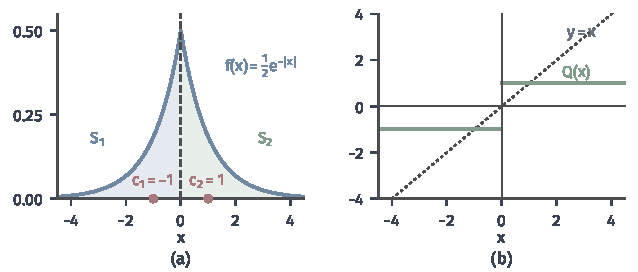
\includegraphics[width=108mm]{figures/07-probability/05-source-coding/matplotlib/quant-two-points/figure.pdf}
 \caption{$\operatorname{Laplace}(0,1)$读数的两点量化器。(a) 蓝线为密度$f$，浅蓝与浅绿分别是区域$S_1=(-\infty,0)$与$S_2=[0,\infty)$，红点为重构值$c_1=-1$、$c_2=1$，虚线为区域边界。(b) 绿线为$Q(x)$，点线为$y=x$；同一横坐标处二者的竖直距离就是误差。}
 \label{fig:quant-two-points}
\end{BookInlineFigure}

最好的重构值依赖于失真函数。若改用绝对误差$d(x,\hat{x})=\lvert x-\hat{x}\rvert$，一个区域内最好的代表值不再是条件均值，而是条件中位数：均值使平方误差最小，中位数使绝对误差最小。在$X\geq0$的条件下，$\operatorname{Exp}(1)$的中位数是$\ln2\approx0.693$，对$Z\sim\operatorname{Exp}(1)$与$c\geq0$直接积分得
\[
 \mathbb{E}\lvert Z-c\rvert=c-1+2\mathrm{e}^{-c} .
\]
取$c=\ln2$得平均绝对误差$0.693$，取$c=1$得$0.736$。同一个源、同样的两个区域，换一个失真函数，最好的重构值就从$\pm1$移到了$\pm0.693$。

右图也显示了误差的两个特点。读数靠近$\pm1$时误差小，远离时误差随$\lvert x\rvert$线性增长；误差完全由读数决定，没有任何随机性。第~\ref{sec:quant-error}节会专门分析这两点。

\paragraph{描述资源}

量化减少了需要记录的内容，但“减少了多少”有三种不同的计量方法，混用会得出错误的比较。图~\ref{fig:quant-pipeline}把一次记录拆成几个环节：编码器把读数变成索引，索引可以原样写成定长比特串，也可以先经过一次无损编码再传送，接收端恢复索引后由解码器报出重构值。

\begin{BookInlineFigure}
 \centering
 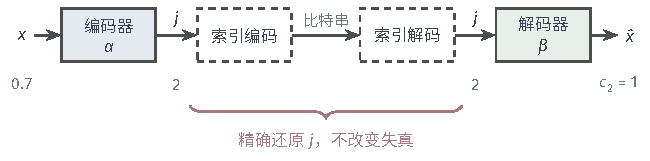
\includegraphics[width=110.1mm]{figures/07-probability/05-source-coding/tikz/quant-pipeline/figure.pdf}
 \caption{量化记录的各个环节。实线框是量化器本身：编码器$\alpha$输出区域索引$j$，解码器$\beta$报出重构值；虚线框是可选的索引编码与解码。下方灰字是两点量化器的例子：读数$0.7$得到索引$2$，重构为$c_2=1$。中间两个环节精确还原索引，因此不改变失真。}
 \label{fig:quant-pipeline}
\end{BookInlineFigure}

第一种计量是重构点数$N$，它决定量化器能区分多少种结果。第二种是\emph{定长索引长度}：每个索引都用同样多的比特写出，需要$\lceil\log_2N\rceil$个比特；$N$是$2$的幂时恰为$\log_2N$。第三种是\emph{平均索引长度}：把索引$J$看作一个离散信源，用第~\ref{chap:lossless-coding}章的唯一可译码描述它，平均长度不小于索引的熵
\[
 H(J)=-\sum_{j=1}^{N}p_j\log_2p_j ,
\]
又可以做到小于$H(J)+1$。由于$H(J)\leq\log_2N$，平均索引长度可以明显短于定长索引长度，尤其当各区域的概率很不均匀时。

处理向量时还要说清是按什么计算的。$d$个读数组成一个向量、用$N$个重构点描述时，每个向量用$\log_2N$个比特，折合每个分量
\begin{equation}
 R=\frac{1}{d}\log_2N
 \label{eq:quant-rate-per-component}
\end{equation}
个比特。比较一个标量量化器和一个二维量化器时，应当在相同的每分量比特数下比较，而不是在相同的点数下比较。

\begin{BookInlineTable}
 \centering
 \begin{tabular}{lll}
  \toprule
  资源 & 计量 & 两点量化器\\
  \midrule
  重构点数 & $N$ & $2$\\
  定长索引长度 & $\lceil\log_2N\rceil$ & $1$ bit\\
  平均索引长度 & 不小于$H(J)$ & $1$ bit\\
  \bottomrule
 \end{tabular}
 \caption{三种描述资源。两点量化器的两个区域概率都是$\tfrac12$，三种计量恰好一致；区域概率不均匀时，平均索引长度可以小于定长索引长度。}
 \label{tab:quant-resources}
\end{BookInlineTable}

表~\ref{tab:quant-resources}汇总了这三种计量。它们回答不同的问题：点数决定重构的精细程度，定长长度适合每个读数必须占用固定存储的场合，平均长度适合可以变长记录的场合。第~\ref{sec:quant-index-coding}节将看到，固定点数时用变长记录可以节省长度，而若以平均长度为预算，最优的区域划分也会随之改变。

\paragraph{有限量化器与长块极限}

给定源分布、失真函数、维数$d$和点数$N$，所有$N$点量化器中平均失真的下确界
\[
 D_N^{*}=\inf_{Q:\,N\text{点}}D(Q)
\]
是有限量化所能达到的最好水平。它依赖于一次联合处理多少个读数。同样是每个读数1 bit，逐个读数用两点量化器，与把两个读数作为二维向量用四点量化器，后者的选择范围包含前者（取两个两点量化器的乘积即可），因此不会更差，往往还更好；第~\ref{sec:quant-vector}节会给出具体例子。

把越来越长的读数块放在一起描述，每分量的最低失真还会继续下降。第~\ref{chap:rate-distortion}章研究这一极限：对方差为$\sigma^{2}$的高斯读数，允许任意长的块时，每个读数1 bit可以把均方误差降到$\sigma^{2}/4$，而逐个读数的最好两点量化器（阈值为零、重构值为$\pm\sigma\sqrt{2/\pi}$）只能达到$(1-2/\pi)\sigma^{2}\approx0.363\sigma^{2}$。所以本章算出的有限量化器失真，是具体方案在给定维数和点数下的表现，不等于给定码率下所有长块编码的最小失真；两者的差距正是下一章要衡量的量。
